\documentclass[
english,
%handout, % enable this switch in order to produce handouts
]{beamer}

\mode<handout>{
  \usepackage{pgf}
  \usepackage{pgfpages}
  \pgfpagesuselayout{2 on 1}[a4paper,border shrink=5mm]
}
\mode<presentation>{
  \usetheme{Juelich}
}
\graphicspath{{img/}}

\usepackage[english]{babel}
\usepackage[scaled]{helvet}
\usepackage[latin1]{inputenc}
\usepackage[T1]{fontenc}
\usepackage{caption}
\usepackage{subcaption}
\usepackage{tikz}
\usepackage{array}
\usepackage{pifont}
\usepackage{braket}
\usepackage{blkarray}
\usetikzlibrary{shapes,arrows}

\renewcommand{\emph}[1]{\structure{#1}}
\def\Put(#1,#2)#3{\makebox(0,0){\put(#1,#2){#3}}}

% Bold vectors
\renewcommand{\vec}[1]{\mathbf{#1}}

% Complex conjugate
\newcommand{\conj}[1]{\overline{#1}}

\title{\LARGE{Calculations of atomic multiplets across the periodic table}}
\subtitle{\normalsize{Master's Thesis}}
\author{Qian Zhang \and Prof.\ Dr.\ Erik Koch}
\institute{\\German Research School for Simulation Sciences \and RWTH Aachen University}
\date{14 October 2014}

\begin{document}
\maketitle

\begin{frame}[t]
  \frametitle{Outline}
  \begin{enumerate}
    \item Introduction
    \item The one-electron problem
    \item The many-electron problem (mean-field approximation)
    \item Construction of multiplet states
    \item Spin-orbit coupling
    \item Conclusion
  \end{enumerate}
\end{frame}
\begin{frame}[t]
  \frametitle{Introduction}
  \begin{columns}
    \begin{column}{0.6\textwidth}
    Imagine our solar system...
    
    \vspace{1em}
    \includegraphics[width=\textwidth]{solar} \\
    \scriptsize (Image from NASA)
    \end{column}
    \begin{column}{0.35\textwidth}
      \centering
      $\vec{F} = m\vec{a}$
      \begin{alignat*}{3}
      & \text{Mercury:} \quad && \vec{r}_1(t) \\
      & \text{Venus:}   \quad && \vec{r}_2(t) \\
      & \text{Earth:}   \quad && \vec{r}_3(t) \\
      & \text{Mars:}    \quad && \vec{r}_4(t) \\
      & && \vdots
      \end{alignat*}
      \pause Analytical solution: \alert{$\textrm{\ding{55}}$} \\
      Numerical solution: \emph{$\textrm{\ding{51}}$}
    \end{column}
  \end{columns}
\end{frame}

\begin{frame}[t]
  \frametitle{Introduction}
  \begin{columns}
    \begin{column}{0.35\textwidth}
    \makebox{Scaling down to $10^{-10}$ meters...}
    
    \vspace{1em}
    \includegraphics[width=\textwidth]{atom} \\
    \scriptsize (Image from Wikipedia)
    \end{column}
    \begin{column}{0.6\textwidth}
      \[H \Psi = E \Psi\]
      \[H = \sum_{i=1}^N \left[ -\frac{1}{2} \nabla_i^2 - \frac{Z}{r_i} \right] + \sum_{i<j}^N \frac{1}{|\vec{r}_i - \vec{r}_j|}\]
      \centering
      Many-electron wave function
      \[\Psi(\vec{r}_1,\vec{r}_2,\ldots,\vec{r}_N)\]
      
      \pause Analytical solution: \alert{$\textrm{\ding{55}}$} \\
      Numerical solution: \alert{$\textrm{\ding{55}}$}
      
      \vspace{1em}
      \pause \emph{$\boxed{\text{Approximations!}}$}
    \end{column}
  \end{columns}
\end{frame}



\begin{frame}[t]
  \frametitle{One-electron problem}
  For $N=1$
  \[ \left[ -\frac{1}{2} \nabla^2 + V(r) \right] \varphi = E \varphi \]
  Separation of variables:
  \[ \varphi(r,\theta,\phi) = R(r)Y(\theta,\phi) \]
  \begin{eqnarray*}
    \text{Angular part} & \emph{Y(\theta,\phi)} & \text{Easy, spherical harmonics} \\
    \text{Radial part} & \emph{R(r)} & \text{Difficult, \alert{our task}}
  \end{eqnarray*}
\end{frame}

\begin{frame}[t]
  \frametitle{One-electron problem}
  \footnotesize
  Angular equation
  \[\frac{1}{\sin{\theta}} \frac{\partial}{\partial \theta} \left( \sin{\theta} \frac{\partial Y}{\partial \theta} \right) + \frac{1}{\sin^2{\theta}} \frac{\partial^2 Y}{\partial \phi^2} = -l(l+1) Y\]
  
  \vspace{-1.6em}
  \pause
  \begin{center}
  \begin{tabular}{c c c c c}
  & & \includegraphics[width=0.15\textwidth,trim={0 3cm 0 -2cm},clip]{00} & & \\
  & \includegraphics[width=0.15\textwidth,trim={0 3cm 0 -2cm},clip]{1m1} & \includegraphics[width=0.15\textwidth,trim={0 3cm 0 -2cm},clip]{10} & \includegraphics[width=0.15\textwidth,trim={0 3cm 0 -2cm},clip]{1p1} & \\
  \includegraphics[width=0.15\textwidth,trim={0 3cm 0 -2cm},clip]{2m2} & \includegraphics[width=0.15\textwidth,trim={0 3cm 0 -2cm},clip]{2m1} & \includegraphics[width=0.15\textwidth,trim={0 3cm 0 -2cm},clip]{20} & \includegraphics[width=0.15\textwidth,trim={0 3cm 0 -2cm},clip]{2p1} & \includegraphics[width=0.15\textwidth,trim={0 3cm 0 -2cm},clip]{2p2}
  \end{tabular}
  \end{center}
  
  \Put(180,250){\emph{
  $\boxed{\begin{aligned}
  & \text{Spherical harmonics: } Y_{lm}(\theta,\phi) \\
  & l = 0,1,\ldots \qquad m = -l,\ldots,l
  \end{aligned}}$}}
\end{frame}

\begin{frame}[t]
  \frametitle{One-electron problem}
  \footnotesize
  Define $u(r) \equiv rR(r)$, \emph{radial equation}
  \[\boxed{-\frac{1}{2} \frac{d^2u}{dr^2} + \left[ V(r) + \frac{l(l+1)}{2r^2} \right] u = E u}\]
  where $V(r)=-Z/r$
  \pause
  \setcounter{subfigure}{0}
  \begin{figure}[h!]
  \centering
  \subfloat[][$Z=1$]{\includegraphics[width=0.325\textwidth]{Z1}}
  \subfloat[][$Z=2$]{\includegraphics[width=0.325\textwidth]{Z2}}
  \subfloat[][$Z=3$]{\includegraphics[width=0.325\textwidth]{Z3}}
  \end{figure}
\end{frame}

\begin{frame}[t]
  \frametitle{Logarithmic grid}
  \footnotesize
  Construct a \emph{logarithmic} grid,
  $ 0 < r_0 < \cdots < r_{n-1} < \infty $, where
  \[r_i = \frac{1}{Z} e^{x_i}\]
  \begin{center}
  \setlength{\unitlength}{5pt}
  \begin{picture}(53.6518,0)
  \put(0,0){\line(1,0){53.6518}}
  \put(0,0){\line(0,1){1}}
  \put(0.2216,0){\line(0,1){1}}
  \put(0.4923,0){\line(0,1){1}}
  \put(0.8229,0){\line(0,1){1}}
  \put(1.2268,0){\line(0,1){1}}
  \put(1.7200,0){\line(0,1){1}}
  \put(2.3224,0){\line(0,1){1}}
  \put(3.0583,0){\line(0,1){1}}
  \put(3.9570,0){\line(0,1){1}}
  \put(5.0547,0){\line(0,1){1}}
  \put(6.3954,0){\line(0,1){1}}
  \put(8.0330,0){\line(0,1){1}}
  \put(10.0332,0){\line(0,1){1}}
  \put(12.4762,0){\line(0,1){1}}
  \put(15.4601,0){\line(0,1){1}}
  \put(19.1046,0){\line(0,1){1}}
  \put(23.5561,0){\line(0,1){1}}
  \put(28.9931,0){\line(0,1){1}}
  \put(35.6339,0){\line(0,1){1}}
  \put(43.7449,0){\line(0,1){1}}
  \put(53.6518,0){\line(0,1){1}}
  \put(-0.5,-2){$r_0$}
  \put(53.1518,-2){$r_{n-1}$}
  \end{picture}
  \end{center}
  and $x$ is a \emph{uniformly} distributed grid
  \[ x_i = x_0 + i \Delta x \]
  \begin{center}
  \setlength{\unitlength}{5pt}
  \begin{picture}(53.6520,0)
  \put(0,0){\line(1,0){53.6520}}
  \put(0,0){\line(0,1){1}}
  \put(2.6826,0){\line(0,1){1}}
  \put(5.3652,0){\line(0,1){1}}
  \put(8.0478,0){\line(0,1){1}}
  \put(10.7304,0){\line(0,1){1}}
  \put(13.4130,0){\line(0,1){1}}
  \put(16.0956,0){\line(0,1){1}}
  \put(18.7782,0){\line(0,1){1}}
  \put(21.4608,0){\line(0,1){1}}
  \put(24.1434,0){\line(0,1){1}}
  \put(26.8260,0){\line(0,1){1}}
  \put(29.5086,0){\line(0,1){1}}
  \put(32.1912,0){\line(0,1){1}}
  \put(34.8738,0){\line(0,1){1}}
  \put(37.5564,0){\line(0,1){1}}
  \put(40.2390,0){\line(0,1){1}}
  \put(42.9216,0){\line(0,1){1}}
  \put(45.6042,0){\line(0,1){1}}
  \put(48.2868,0){\line(0,1){1}}
  \put(50.9694,0){\line(0,1){1}}
  \put(53.6520,0){\line(0,1){1}}
  \put(-0.5,-2){$x_0$}
  \put(53.1520,-2){$x_{n-1}$}
  \end{picture}
  \end{center}
\end{frame}

\begin{frame}[t]
  \frametitle{Logarithmic grid}
  \footnotesize
  \setcounter{subfigure}{0}
  \begin{figure}[h!]
  \centering
  \subfloat[][$Z=1$]{\includegraphics[width=0.325\textwidth]{Z1t}}
  \subfloat[][$Z=2$]{\includegraphics[width=0.325\textwidth]{Z2t}}
  \subfloat[][$Z=3$]{\includegraphics[width=0.325\textwidth]{Z3t}}
  \end{figure}
  Rescale $\tilde{u} \equiv u/\sqrt{r}$, the \emph{transformed radial equation}
  \[ -\frac{1}{2} \frac{d^2\tilde{u}}{dx^2} + \left[ r^2 V(r) + \frac{1}{2} \Big(l+\frac{1}{2}\Big)^2 \right] \tilde{u} = r^2 E \tilde{u} \]
\end{frame}


% \begin{frame}[t]
%   \frametitle{Numerov's method}
%   \footnotesize
%   Finite difference
%   \[\frac{d^2\tilde{u}}{dx^2} = \frac{\tilde{u}_{i+1} - 2\tilde{u}_i + \tilde{u}_{i-1}}{\Delta x^2} + \mathcal{O}(\Delta x^2)\]
%   \pause
%   \emph{Numerov's method}
%   \[\frac{d^2\tilde{u}}{dx^2} = \frac{\tilde{u}_{i+1} - 2\tilde{u}_i + \tilde{u}_{i-1}}{\Delta x^2} - \frac{1}{12}\frac{\tilde{u}_{i+1}^{''} - 2\tilde{u}_i^{''} + \tilde{u}_{i-1}^{''}}{\Delta x^2}\Delta x^2 + \mathcal{O}(\Delta x^4)\]
%   \pause
%   Use the original ODE
%   \[\tilde{u}_i^{''} = -2 k_i^2 \tilde{u_i}
%   \quad \text{and} \quad k_i^2 \equiv r_i^2 E - r_i^2 V(r_i) - \frac{1}{2} \Big(l+\frac{1}{2}\Big)^2\]
%   \pause
%   3-point \alert{recursion}!
%   \[\tilde{u}_{i\pm1} = \frac{(2-\frac{5\Delta x^2}{3}k_i^2)\tilde{u}_i - (1+\frac{\Delta x^2}{6}k_{i\mp1}^2)\tilde{u}_{i\mp1}}{1+\frac{\Delta x^2}{6}k_{i\pm1}^2}\]
% \end{frame}

\begin{frame}[t]
  \frametitle{The shooting and matching methods}
  \footnotesize
%   \begin{tabular}{|c|c|}
%     \hline
%     & Initialization \\ \hline
%     Forward &
%     $\begin{aligned}
%     \smash[b]{\vphantom{\Big|}}
%     \tilde{u}_0 & = r_0^{l+1} / \sqrt{r_0} \\
%     \tilde{u}_1 & = r_1^{l+1} / \sqrt{r_1}
%     \smash[t]{\vphantom{\Big|}}
%     \end{aligned}$ \\ \hline
%     Backward &
%     $\begin{aligned}
%     \smash[b]{\vphantom{\Big|}}
%     \tilde{u}_{n-1} & = e^{-\beta r_{n-1}} / \sqrt{r_{n-1}} \\
%     \tilde{u}_{n-2} & = e^{-\beta r_{n-2}} / \sqrt{r_{n-2}}
%     \smash[t]{\vphantom{\Big|}}
%     \end{aligned}$ \\
%     \hline
%   \end{tabular}
  \emph{Numerov's method}
  
  \vspace{1em}
  $\tilde{u}_{i\pm1} = \dfrac{(2-\frac{5\Delta x^2}{3}k_i^2)\tilde{u}_i - (1+\frac{\Delta x^2}{6}k_{i\mp1}^2)\tilde{u}_{i\mp1}}{1+\frac{\Delta x^2}{6}k_{i\pm1}^2}$
  \Put(5,0){\includegraphics[width=0.4\textwidth]{r1r2}} \pause
  
  \vspace{4em}
  \setcounter{subfigure}{0}
  \begin{figure}[h!]
  \centering
  \subfloat[][$E=-0.6$]{\includegraphics[width=0.325\textwidth]{E06}} \pause
  \subfloat[][$E=-0.4$]{\includegraphics[width=0.325\textwidth]{E04}} \pause
  \subfloat[][$E=-0.5$]{\includegraphics[width=0.325\textwidth]{E05}}
  \end{figure}
\end{frame}

\begin{frame}[t]
  \frametitle{Numerical and exact eigen-energy comparison}
  \footnotesize
  \centering
  \begin{tabular}{ c | c | r | r | r | r }
    \hline
  Elem & Orbital & Numerical & Exact & Abs Error & Rel Error \\ \hline \hline
    H &  $1s$  &  $-0.500000$  &  $-0.500000$  &  0.000000  &  0.000000 \\  \hline
    C &  $1s$  &  $-18.000002$  &  $-18.000000$  &  0.000002  &  0.000000 \\ 
      &  $2s$  &  $-4.499999$  &  $-4.500000$  &  0.000001  &  0.000000 \\ 
      &  $2p$  &  $-4.500001$  &  $-4.500000$  &  0.000001  &  0.000000 \\  \hline
  Fe &  $1s$  &  $-338.000032$  &  $-338.000000$  &  0.000032  &  0.000000 \\ 
      &  $2s$  &  $-84.499984$  &  $-84.500000$  &  0.000016  &  0.000000 \\ 
      &  $2p$  &  $-84.500012$  &  $-84.500000$  &  0.000012  &  0.000000 \\ 
      &  $3s$  &  $-37.555556$  &  $-37.555556$  &  0.000000  &  0.000000 \\ 
      &  $3p$  &  $-37.555556$  &  $-37.555556$  &  0.000000  &  0.000000 \\
      &  $3d$  &  $-37.555555$  &  $-37.555556$  &  0.000001  &  0.000000 \\
      &  $4s$  &  $-21.125000$  &  $-21.125000$  &  0.000000  &  0.000000 \\
    \hline
  \end{tabular}
  
  \emph{\[\boxed{\text{One electron only!}}\]}
\end{frame}

\begin{frame}[t]
  \frametitle{The many-electron problem}
  Many-electron Schr{\"o}dinger equation
  \[\left\{\sum_{i=1}^N \left[ -\frac{1}{2} \nabla_i^2 - \frac{Z}{r_i} \right] + \sum_{i<j}^N \frac{1}{|\vec{r}_i - \vec{r}_j|}\right\} \Psi = E \Psi\] \pause
  \begin{itemize}
      \item {Analytical solution: \alert{$\textrm{\ding{55}}$}}
      \item {Numerical solution: \alert{$\textrm{\ding{55}}$}}
      \item {We use \emph{self-consistent field (SCF)} approximation}
  \end{itemize}
\end{frame}

\begin{frame}[t]
  \frametitle{The many-electron problem}
  \emph{Hartree} ansatz
  \[ \Psi(\vec{r}_1,\vec{r}_2,\ldots,\vec{r}_N) \approx \varphi_1(\vec{r}_1)\varphi_2(\vec{r}_2)\ldots\varphi_N(\vec{r}_N) \]
  \emph{Mean-field} approximation
  \begin{align*}
  H & = \sum_{i=1}^N \left[ -\frac{1}{2} \nabla_i^2 - \frac{Z}{r_i} \right] + \underbrace{\sum_{i<j}^N \frac{1}{|\vec{r}_i - \vec{r}_j|}}_{\text{\alert{Trouble maker}}} \\
  H & = \sum_{i=1}^N \left[ -\frac{1}{2} \nabla_i^2 - \frac{Z}{r_i} \right] + \underbrace{V_\text{Hartree}(r)}_{\text{\emph{Hartree potential}}}
  \end{align*}
\end{frame}

\begin{frame}[t]
  \frametitle{Self-consistent iteration}
  \footnotesize
  \emph{Many-electron} problem $\rightarrow$ Many \emph{one-electron} problems
  \[ \boxed{-\frac{1}{2} \frac{d^2u_i}{dr^2} + \left[ V_{\text{ext}}(r) +  \emph{V_{\text{Hartree}}(r)} + \frac{l(l+1)}{2r^2} \right] u_i = E_i u_i} \] \pause
  Chicken or the egg problem!
  \scriptsize
  \tikzstyle{cloud}    = [ellipse, draw, text width=4.0em, text badly centered, minimum height=2em]
  \tikzstyle{block}    = [rectangle, draw, rounded corners, text width=4.5em, text badly centered, minimum height=4em]
  \tikzstyle{decision} = [diamond, draw, text width=4.5em, text badly centered, aspect=1.5]
  \tikzstyle{line}     = [draw, -triangle 45]
  \Put(-130,-170){
  \begin{tikzpicture}[node distance = 9em, auto]
  % Place nodes
  \node [cloud] (init) {initial potential};
  \node [block, right of=init] (orbital) {compute \emph{$\{u_i(r)\}$}};
  \node [block, right of=orbital] (potential) {compute \emph{$V_{\text{Hartree}}(r)$}};
  \node [block, below of=potential, node distance=5em] (update) {update \emph{$V_{\text{Hartree}}(r)$}};
  \node [decision, right of=potential] (converge) {converged?};
  \node [cloud, right of=converge, text width=2.5em,] (stop) {stop};
  % Draw edges
  \path [line] (init) -- (orbital);
  \path [line] (orbital) -- (potential);
  \path [line] (potential) -- (converge);
  \path [line] (converge) |- node [near start] {no} (update);
  \path [line] (update) -| (orbital);
  \path [line] (converge) -- node {yes}(stop);
  \end{tikzpicture}
  }
\end{frame}

\begin{frame}[t]
  \frametitle{JavaScript demonstration}
  \footnotesize
  \centering
  \includegraphics[width=0.8\textwidth]{js1}
  \[\texttt{www.cond-mat.de/sims/multiplet}\]
\end{frame}

\begin{frame}[t]
  \def\sqbox{
    \setlength{\unitlength}{1.5pt}
    \begin{picture}(10,10)
      \thicklines
      \color{red}
      \put(0,1){\line(1,0){12}}
      \put(12,1){\line(0,1){9}}
      \put(12,10){\line(-1,0){12}}
      \put(0,10){\line(0,-1){9}}
    \end{picture}
  }
  \frametitle{Comparison to NIST results}
  \footnotesize
  \centering
  \begin{tabular}{ c | c | r | r | r | r }
    \hline
    Elem & Orbital & My results & NIST results & Abs Error & Rel Error \\ \hline \hline
    H &  $1s^1$  &  $-0.233471$  &  $-0.233471$  &  0.000000  &  0.000000 \\  \hline
    C &  $1s^2$  &  $-9.947725$  &  $-9.947718$  &  0.000007  &  0.000001 \\ 
      &  $2s^2$  &  $-0.500866$  &  $-0.500866$  &  0.000000  &  0.000000 \\ 
      &  $2p^2$  &  $-0.199186$  &  $-0.199186$  &  0.000000  &  0.000000 \\ \hline
  Fe &  $1s^2$  &  $-254.225334$  &  $-254.225505$  &  0.000171  &  0.000001 \\ 
      &  $2s^2$  &  $-29.564863$  &  $-29.564860$  &  0.000003  &  0.000000 \\ 
      &  $2p^6$  &  $-25.551762$  &  $-25.551766$  &  0.000004  &  0.000000 \\ 
      &  $3s^2$  &  $-3.360622$  &  $-3.360621$  &  0.000001  &  0.000000 \\ 
      &  $3p^6$  &  $-2.187521$  &  $-2.187523$  &  0.000002  &  0.000001 \\
      &  $3d^6$  &  $-0.295047$  &  $-0.295049$  &  0.000002  &  0.000007 \\
      &  $4s^2$  &  $-0.197976$  &  $-0.197978$  &  0.000002  &  0.000010 \\
    \hline
  \end{tabular}
  
  \emph{\[\boxed{\text{Many-electron, mean-field!}}\]} \pause  
  
  \Put(37,258){\sqbox}
\end{frame}

\begin{frame}[t]
  \frametitle{Open shell problem}
  Imagine the following problem:
  
  \vspace{0.5em}
  \begin{equation*}
  \begin{array}{c|c|c|c|}
  \multicolumn{1}{c}{} & \multicolumn{1}{c}{\phantom{,}1\phantom{,}} & \multicolumn{1}{c}{\phantom{,}0\phantom{,}} & \multicolumn{1}{c}{-1} \\ \cline{2-4}
  \uparrow &  &  &  \\ \cline{2-4}
  \downarrow &  &  &  \\
  \cline{2-4}
  \multicolumn{1}{c}{}
  \end{array}
  \qquad \text{and} \qquad
  \bullet \ \bullet \qquad
  \end{equation*}
  \Put(90,20){\emph{$p$ shell}}
  \Put(185,20){\emph{2 electrons}}
\end{frame}

\begin{frame}[t]
  \frametitle{Open shell problem}
  \footnotesize
  \begin{center}
  \vspace{-0.5em}
  \begin{tabular}{|c|c|c|}
  \hline
  $\bullet$ & $\bullet$ & $\phantom{\bullet}$ \\ \hline
  &  &  \\
  \hline
  \end{tabular}
  \begin{tabular}{|c|c|c|}
  \hline
  $\bullet$ & $\phantom{\bullet}$ & $\bullet$ \\ \hline
  &  &  \\
  \hline
  \end{tabular}
  \begin{tabular}{|c|c|c|}
  \hline
  $\bullet$ & $\phantom{\bullet}$ & $\phantom{\bullet}$ \\ \hline
  $\bullet$ &  &  \\
  \hline
  \end{tabular}
  \begin{tabular}{|c|c|c|}
  \hline
  $\bullet$ & $\phantom{\bullet}$ & $\phantom{\bullet}$ \\ \hline
  & $\bullet$ &  \\
  \hline
  \end{tabular}
  \begin{tabular}{|c|c|c|}
  \hline
  $\bullet$ & $\phantom{\bullet}$ & $\phantom{\bullet}$ \\ \hline
  &  & $\bullet$ \\
  \hline
  \end{tabular} \\
  \vspace{0.5em}
  \begin{tabular}{|c|c|c|}
  \hline
  $\phantom{\bullet}$ & $\bullet$ & $\bullet$ \\ \hline
  &  &  \\
  \hline
  \end{tabular}
  \begin{tabular}{|c|c|c|}
  \hline
  $\phantom{\bullet}$ & $\bullet$ & $\phantom{\bullet}$ \\ \hline
  $\bullet$ &  &  \\
  \hline
  \end{tabular}
  \begin{tabular}{|c|c|c|}
  \hline
  $\phantom{\bullet}$ & $\bullet$ & $\phantom{\bullet}$ \\ \hline
  & $\bullet$ &  \\
  \hline
  \end{tabular}
  \begin{tabular}{|c|c|c|}
  \hline
  $\phantom{\bullet}$ & $\bullet$ & $\phantom{\bullet}$ \\ \hline
  &  & $\bullet$ \\
  \hline
  \end{tabular}
  \begin{tabular}{|c|c|c|}
  \hline
  $\phantom{\bullet}$ & $\phantom{\bullet}$ & $\bullet$ \\ \hline
  $\bullet$ &  &  \\
  \hline
  \end{tabular} \\
  \vspace{0.5em}
  \begin{tabular}{|c|c|c|}
  \hline
  $\phantom{\bullet}$ & $\phantom{\bullet}$ & $\bullet$ \\ \hline
  & $\bullet$ &  \\
  \hline
  \end{tabular}
  \begin{tabular}{|c|c|c|}
  \hline
  $\phantom{\bullet}$ & $\phantom{\bullet}$ & $\bullet$ \\ \hline
  &  & $\bullet$ \\
  \hline
  \end{tabular}
  \begin{tabular}{|c|c|c|}
  \hline
  $\phantom{\bullet}$ & $\phantom{\bullet}$ & $\phantom{\bullet}$ \\ \hline
  $\bullet$ & $\bullet$ &  \\
  \hline
  \end{tabular}
  \begin{tabular}{|c|c|c|}
  \hline
  $\phantom{\bullet}$ & $\phantom{\bullet}$ & $\phantom{\bullet}$ \\ \hline
  $\bullet$ &  & $\bullet$ \\
  \hline
  \end{tabular}
  \begin{tabular}{|c|c|c|}
  \hline
  $\phantom{\bullet}$ & $\phantom{\bullet}$ & $\phantom{\bullet}$ \\ \hline
  & $\bullet$ & $\bullet$ \\
  \hline
  \end{tabular}
  \end{center}
  Which configuration has the highest energy?
  
  \Put(230,-100){\includegraphics[width=0.1\textwidth]{quest}} \pause
  \alert{\[\frac{1}{\sqrt{3}}
  \begin{array}{|c|c|c|}
  \hline
  & \phantom{\bullet} & \bullet \\ \hline
  \bullet &  &  \\
  \hline
  \end{array}
  - \frac{1}{\sqrt{3}}
  \begin{array}{|c|c|c|}
  \hline
  \phantom{\bullet} & \bullet & \phantom{\bullet} \\ \hline
  & \bullet &  \\
  \hline
  \end{array}
  + \frac{1}{\sqrt{3}}
  \begin{array}{|c|c|c|}
  \hline
  \bullet & \phantom{\bullet} & \\ \hline
  &  & \bullet \\
  \hline
  \end{array}\qquad\qquad\qquad\qquad\qquad\]}
\end{frame}

\begin{frame}[t]
  \frametitle{Coulomb repulsion Hamiltonian}
  \footnotesize
  Revisit our \alert{trouble maker}
  \[ H_U = \sum_{i<j}^N \frac{1}{|\vec{r}_i - \vec{r}_j|} \]
  \emph{Second quantization}
  \begin{equation*}
  H_U = \frac{1}{2} \sum_{\alpha,\beta,\gamma,\delta} U_{\alpha\beta\gamma\delta} c_\alpha^\dag c_\beta^\dag c_\gamma c_\delta
  \end{equation*}
  \begin{align*}
  \alpha & = \{n_1,\,l_1,\,m_1,\,\sigma_1\} \\
  \beta  & = \{n_2,\,l_2,\,m_2,\,\sigma_2\} \\
  \gamma & = \{n_3,\,l_3,\,m_3,\,\sigma_3\} \\
  \delta & = \{n_4,\,l_4,\,m_4,\,\sigma_4\}
  \end{align*}
\end{frame}

\begin{frame}[t]
  \frametitle{Coulomb repulsion Hamiltonian}
  \footnotesize
  Coulomb repulsion \emph{matrix element}
  \begin{align*} & U_{\alpha\beta\gamma\delta} = \\
  & \delta_{\sigma_1\sigma_4} \delta_{\sigma_2\sigma_3} \int d^3r_1 \int d^3r_2 \,
  \conj{\varphi_{n_1l_1m_1}}(\vec{r}_1) \conj{\varphi_{n_2l_2m_2}}(\vec{r}_2)
  \frac{1}{|\vec{r}_1 - \vec{r}_2|}
  \varphi_{n_3l_3m_3}(\vec{r}_2) \varphi_{n_4l_4m_4}(\vec{r}_1) \end{align*} \pause
  Multipole expansion
  \[\frac{1}{|\vec{r}_1-\vec{r}_2|} = \sum_{k=0}^\infty \underbrace{\frac{r_<^k}{r_>^{k+1}}}_{\emph{\text{Radial part}}} \frac{4\pi}{2k+1}
    \sum_{\mu=-k}^k \underbrace{\conj{Y_{k\mu}}(\theta_1,\phi_1) Y_{k\mu}(\theta_2,\phi_2)}_{\emph{\text{Angular part}}}\]
\end{frame}

\begin{frame}[t]
  \frametitle{Coulomb repulsion Hamiltonian}
  \footnotesize
  The \emph{radial} part
  \[
  R^{(k)}(n_1l_1,n_2l_2,n_3l_3,n_4l_4) =
  \int_0^\infty dr_1 \int_0^\infty dr_2\, \conj{u_{n_1l_1}}(r_1) \conj{u_{n_2l_2}}(r_2)
  \frac{r_<^k}{r_>^{k+1}} u_{n_3l_3}(r_2) u_{n_4l_4}(r_1)
  \]
  The \emph{angular} part
  
  \vspace{1em}
  $A^{(k)}(l_1m_1,l_2m_2,l_3m_3,l_4m_4) =$
  \begin{align*}
  \sum_{\mu=-k}^k
  & \int_0^{2\pi}d\phi_1 \int_0^{\pi}d\theta_1\,\sin{\theta_1}\,
    \conj{Y_{l_1m_1}}(\theta_1,\phi_1) \conj{Y_{k\mu}}(\theta_1,\phi_1) Y_{l_4m_4}(\theta_1,\phi_1) \nonumber \\
  & \int_0^{2\pi}d\phi_2 \int_0^{\pi}d\theta_2\,\sin{\theta_2}\,
    \conj{Y_{l_2m_2}}(\theta_2,\phi_2) Y_{k\mu}(\theta_2,\phi_2) Y_{l_3m_3}(\theta_2,\phi_2)
  \end{align*} \pause
  
  \Put(170,225){\emph{$\boxed{\text{Slater-Condon parameters}}$}}
  \Put(170,25){\emph{$\boxed{\text{Gaunt coefficients}}$}}
\end{frame}

\begin{frame}[t]
  \frametitle{Setting up basis and Hamiltonian}
  \footnotesize
  Set up \emph{basis}
  \begin{center}
  \vspace{-0.5em}
  \begin{tabular}{|c|c|c|}
  \hline
  $\bullet$ & $\bullet$ & $\phantom{\bullet}$ \\ \hline
  &  &  \\
  \hline
  \end{tabular}
  \begin{tabular}{|c|c|c|}
  \hline
  $\bullet$ & $\phantom{\bullet}$ & $\bullet$ \\ \hline
  &  &  \\
  \hline
  \end{tabular}
  \begin{tabular}{|c|c|c|}
  \hline
  $\bullet$ & $\phantom{\bullet}$ & $\phantom{\bullet}$ \\ \hline
  $\bullet$ &  &  \\
  \hline
  \end{tabular}
  \begin{tabular}{|c|c|c|}
  \hline
  $\bullet$ & $\phantom{\bullet}$ & $\phantom{\bullet}$ \\ \hline
  & $\bullet$ &  \\
  \hline
  \end{tabular}
  \begin{tabular}{|c|c|c|}
  \hline
  $\bullet$ & $\phantom{\bullet}$ & $\phantom{\bullet}$ \\ \hline
  &  & $\bullet$ \\
  \hline
  \end{tabular} \\
  \vspace{0.5em}
  \begin{tabular}{|c|c|c|}
  \hline
  $\phantom{\bullet}$ & $\bullet$ & $\bullet$ \\ \hline
  &  &  \\
  \hline
  \end{tabular}
  \begin{tabular}{|c|c|c|}
  \hline
  $\phantom{\bullet}$ & $\bullet$ & $\phantom{\bullet}$ \\ \hline
  $\bullet$ &  &  \\
  \hline
  \end{tabular}
  \begin{tabular}{|c|c|c|}
  \hline
  $\phantom{\bullet}$ & $\bullet$ & $\phantom{\bullet}$ \\ \hline
  & $\bullet$ &  \\
  \hline
  \end{tabular}
  \begin{tabular}{|c|c|c|}
  \hline
  $\phantom{\bullet}$ & $\bullet$ & $\phantom{\bullet}$ \\ \hline
  &  & $\bullet$ \\
  \hline
  \end{tabular}
  \begin{tabular}{|c|c|c|}
  \hline
  $\phantom{\bullet}$ & $\phantom{\bullet}$ & $\bullet$ \\ \hline
  $\bullet$ &  &  \\
  \hline
  \end{tabular} \\
  \vspace{0.5em}
  \begin{tabular}{|c|c|c|}
  \hline
  $\phantom{\bullet}$ & $\phantom{\bullet}$ & $\bullet$ \\ \hline
  & $\bullet$ &  \\
  \hline
  \end{tabular}
  \begin{tabular}{|c|c|c|}
  \hline
  $\phantom{\bullet}$ & $\phantom{\bullet}$ & $\bullet$ \\ \hline
  &  & $\bullet$ \\
  \hline
  \end{tabular}
  \begin{tabular}{|c|c|c|}
  \hline
  $\phantom{\bullet}$ & $\phantom{\bullet}$ & $\phantom{\bullet}$ \\ \hline
  $\bullet$ & $\bullet$ &  \\
  \hline
  \end{tabular}
  \begin{tabular}{|c|c|c|}
  \hline
  $\phantom{\bullet}$ & $\phantom{\bullet}$ & $\phantom{\bullet}$ \\ \hline
  $\bullet$ &  & $\bullet$ \\
  \hline
  \end{tabular}
  \begin{tabular}{|c|c|c|}
  \hline
  $\phantom{\bullet}$ & $\phantom{\bullet}$ & $\phantom{\bullet}$ \\ \hline
  & $\bullet$ & $\bullet$ \\
  \hline
  \end{tabular}
  \end{center}
  \begin{equation*}
  \begin{array}{c c c c c c c c c}
  \Ket{110000} & & \Ket{101000} & & \Ket{100100} & & \Ket{100010} & & \Ket{100001} \\
  \Ket{011000} & & \Ket{010100} & & \Ket{010010} & & \Ket{010001} & & \Ket{001100} \\
  \Ket{001010} & & \Ket{001001} & & \Ket{000110} & & \Ket{000101} & & \Ket{000011}
  \end{array}
  \end{equation*}
\end{frame}

\begin{frame}[t]
  \frametitle{Setting up basis and Hamiltonian}
  \footnotesize
  Set up \emph{Hamiltonian}
  \[\Bra{i} H_U \Ket{j} = \Bra{i} \frac{1}{2} \sum_{\alpha,\beta,\gamma,\delta} U_{\alpha\beta\gamma\delta} c_\alpha^\dag c_\beta^\dag c_\gamma c_\delta \Ket{j} \]
  
  \uncover<1>{\Put(10,-262){\includegraphics[width=0.95\textwidth]{Hu}}}
  \uncover<2>{\Put(23,-259){\includegraphics[width=0.95\textwidth]{Huu}}}
\end{frame}

\begin{frame}[t]
  \frametitle{Construction of multiplet states}
  \footnotesize
  Commutation relations
  \[ [H_U,\,\vec{L}]=0 \qquad [H_U,\,\vec{S}]=0 \]
  \begin{equation*}
  [H_U,\,L^2]=0 \qquad [H_U,\,L_z]=0 \qquad
  [H_U,\,S^2]=0 \qquad [H_U,\,S_z]=0
  \end{equation*}
  We can represent an \emph{eigen-vector}
  \[\Ket{L, M_L, S, M_S}\] \pause
  Commutation relations
  \[ [H_U,\,L_\pm]=0 \qquad [H_U,\,S_\pm]=0 \]
  
  \vspace{-1em}
  \emph{\begin{equation*}
  \boxed{
  \begin{aligned}
  & \textbf{Starting from a leading vector, we can construct subsequent} \\
  & \textbf{vectors by applying ladder operators.}
  \end{aligned}
  }
  \end{equation*}}
\end{frame}

\begin{frame}[t]
  \frametitle{Construction of multiplet states}
  \footnotesize
  $M_L$-$M_S$ table
  \begin{center}
  \begin{tabular}{c c|r c c}
        &  &  & $M_S$ & \\
        &  & $-1$ & $0$ & $1$ \\ \hline
        & $\phantom{-}2$ & 0 & 1 & 0 \\
        & $\phantom{-}1$ & 1 & 2 & $\boxed{1}$ \\
  $M_L$ & $\phantom{-}0$ & 1 & 3 & 1 \\
        & $-1$ & 1 & 2 & 1 \\
        & $-2$ & 0 & 1 & 0 \\
  \end{tabular}
  \end{center}
  
  \vspace{-0.5em}
  \begin{center}
  \begin{tabular}{r r r}
  $\phantom{\Ket{1,\phantom{-}1,1,-1}}$ & $\phantom{\Ket{1,\phantom{-}1,1,\phantom{-}0}}$ & $\Ket{1,\phantom{-}1,1,\phantom{-}1}$ \\
  $\phantom{\Ket{1,\phantom{-}0,1,-1}}$ & $\phantom{\Ket{1,\phantom{-}0,1,\phantom{-}0}}$ & $\phantom{\Ket{1,\phantom{-}0,1,\phantom{-}1}}$ \\
  $\phantom{\Ket{1,-1,1,-1}}$ & $\phantom{\Ket{1,-1,1,\phantom{-}0}}$ & $\phantom{\Ket{1,-1,1,\phantom{-}1}}$ \\
  \end{tabular}
  \end{center}
\end{frame}

\begin{frame}[t]
  \frametitle{Construction of multiplet states}
  \footnotesize
  $M_L$-$M_S$ table
  \begin{center}
  \begin{tabular}{c c|r c c}
        &  &  & $M_S$ &  \\
        &  & $-1$ & $0$ & $1$ \\ \hline
        & $\phantom{-}2$ & 0 & 1 & 0  \\
        & $\phantom{-}1$ & $\boxed{1}$ & $\boxed{2}$ & $\boxed{1}$ \\
  $M_L$ & $\phantom{-}0$ & $\boxed{1}$ & $\boxed{3}$ & $\boxed{1}$ \\
        & $-1$ & $\boxed{1}$ & $\boxed{2}$ & $\boxed{1}$ \\
        & $-2$ & 0 & 1 & 0  \\
  \end{tabular}
  \end{center}
  \begin{center}
  \begin{tabular}{r r r}
  $\Ket{1,\phantom{-}1,1,-1}$ & $\Ket{1,\phantom{-}1,1,\phantom{-}0}$ & $\Ket{1,\phantom{-}1,1,\phantom{-}1}$ \\
  $\Ket{1,\phantom{-}0,1,-1}$ & $\Ket{1,\phantom{-}0,1,\phantom{-}0}$ & $\Ket{1,\phantom{-}0,1,\phantom{-}1}$ \\
  $\Ket{1,-1,1,-1}$ & $\Ket{1,-1,1,\phantom{-}0}$ & $\Ket{1,-1,1,\phantom{-}1}$ \\
  \end{tabular}
  \end{center}
  
  \Put(260,65){$\emph{\Large \boxed{{^3P}}}$}
\end{frame}

\begin{frame}[t]
  \frametitle{Construction of multiplet states}
  \footnotesize
  $M_L$-$M_S$ table
  \begin{center}
  \begin{tabular}{c c|r c c}
        &  &  & $M_S$ & \\
        &  & $-1$ & $0$ & $1$ \\ \hline
        & $\phantom{-}2$ & 0 & $\boxed{1}$ & 0 \\
        & $\phantom{-}1$ & 0 & 1 & 0 \\
  $M_L$ & $\phantom{-}0$ & 0 & 2 & 0 \\
        & $-1$ & 0 & 1 & 0 \\
        & $-2$ & 0 & 1 & 0 \\
  \end{tabular}
  \end{center}
  
  \vspace{-0.5em}
  \begin{center}
  \begin{tabular}{r}
  $\qquad\qquad\qquad\Ket{2,\phantom{-}2,0,\phantom{-}0}$
  \end{tabular}
  \end{center}
\end{frame}

\begin{frame}[t]
  \frametitle{Construction of multiplet states}
  \footnotesize
  $M_L$-$M_S$ table
  \begin{center}
  \begin{tabular}{c c|r c c}
        &  &  & $M_S$ & \\
        &  & $-1$ & $0$ & $1$ \\ \hline
        & $\phantom{-}2$ & 0 & $\boxed{1}$ & 0 \\
        & $\phantom{-}1$ & 0 & $\boxed{1}$ & 0 \\
  $M_L$ & $\phantom{-}0$ & 0 & $\boxed{2}$ & 0 \\
        & $-1$ & 0 & $\boxed{1}$ & 0 \\
        & $-2$ & 0 & $\boxed{1}$ & 0 \\
  \end{tabular}
  \end{center}
  \begin{center}
  \begin{tabular}{r}
  $\qquad\qquad\qquad\Ket{2,\phantom{-}2,0,\phantom{-}0}$ \\
  $\qquad\qquad\qquad\Ket{2,\phantom{-}1,0,\phantom{-}0}$ \\
  $\qquad\qquad\qquad\Ket{2,\phantom{-}0,0,\phantom{-}0}$ \\
  $\qquad\qquad\qquad\Ket{2,-1,0,\phantom{-}0}$ \\
  $\qquad\qquad\qquad\Ket{2,-2,0,\phantom{-}0}$ \\
  \end{tabular}
  \end{center}

  \Put(260,105){$\emph{\Large \boxed{{^1D}}}$}
\end{frame}

\begin{frame}[t]
  \frametitle{Construction of multiplet states}
  \footnotesize
  $M_L$-$M_S$ table
  \begin{center}
  \begin{tabular}{c c|r c c}
        &  &  & $M_S$ & \\
        &  & $-1$ & $0$ & $1$ \\ \hline
        & $\phantom{-}2$ & 0 & 0 & 0 \\
        & $\phantom{-}1$ & 0 & 0 & 0 \\
  $M_L$ & $\phantom{-}0$ & 0 & $\boxed{1}$ & 0 \\
        & $-1$ & 0 & 0 & 0 \\
        & $-2$ & 0 & 0 & 0 \\
  \end{tabular}
  \end{center}
  
  \vspace{-0.5em}
  \begin{center}
  \begin{tabular}{r}
  $\qquad\qquad\qquad\Ket{0,\phantom{-}0,0,\phantom{-}0}$ \\
  \end{tabular}
  \end{center}
  
  \Put(260,42){$\emph{\Large \boxed{{^1S}}}$}
\end{frame}

\begin{frame}[t]
  \frametitle{Construction of multiplet states}
  \footnotesize
  Three groups of \emph{eigen-vectors}
  
  \Put(-15,-110){
  \begin{tabular}{|c c c|c|c|}
  \hline
  & $^3P$ &  & $^1D$ & $^1S$  \\ \hline
  &  &  & $\Ket{2,\phantom{-}2,0,\phantom{-}0}$ & \\
  $\Ket{1,\phantom{-}1,1,-1}$ & $\Ket{1,\phantom{-}1,1,\phantom{-}0}$ & $\Ket{1,\phantom{-}1,1,\phantom{-}1}$ & $\Ket{2,\phantom{-}1,0,\phantom{-}0}$ & \\
  $\Ket{1,\phantom{-}0,1,-1}$ & $\Ket{1,\phantom{-}0,1,\phantom{-}0}$ & $\Ket{1,\phantom{-}0,1,\phantom{-}1}$ & $\Ket{2,\phantom{-}0,0,\phantom{-}0}$ & $\Ket{0,\phantom{-}0,0,\phantom{-}0}$ \\
  $\Ket{1,-1,1,-1}$ & $\Ket{1,-1,1,\phantom{-}0}$ & $\Ket{1,-1,1,\phantom{-}1}$ & $\Ket{2,-1,0,\phantom{-}0}$ & \\
  &  &  & $\Ket{2,-2,0,\phantom{-}0}$ & \\
  \hline
  \end{tabular}}
  
  \vspace{8.2em}
  \emph{Multiplet} term symbol
  {\LARGE \emph{\[^{2S+1}L\]}}
\end{frame}

% \begin{frame}[t]
%   \frametitle{Construction of multiplet states}
%   \scriptsize
%   \emph{Ladder operators}
%   \[ L_\pm \Ket{lm} = \alpha_{lm}^\pm \Ket{l,m\pm1} \]
%   
%   \vspace{-2.5em}
%   \begin{align*}
%   \alpha_{lm}^+ & = \sqrt{(l+m+1)(l-m)} \\
%   \alpha_{lm}^- & = \sqrt{(l+m)(l-m+1)}
%   \end{align*}
%   Express eigen-vectors in terms of our 15 basis states
%   \begin{align*}
%   L_-
%   \begin{array}{|c|c|c|}
%   \hline
%   \bullet & \phantom{\bullet} & \phantom{\bullet} \\ \hline
%   \bullet &  &  \\
%   \hline
%   \end{array} & =
%   \sqrt{(1+1)(1-1+1)}
%   \begin{array}{|c|c|c|}
%   \hline
%   \phantom{\bullet} & \bullet & \phantom{\bullet} \\ \hline
%   \bullet &  &  \\
%   \hline
%   \end{array} +
%   \sqrt{(1+1)(1-1+1)}
%   \begin{array}{|c|c|c|}
%   \hline
%   \bullet & \phantom{\bullet} & \phantom{\bullet} \\ \hline
%   & \bullet &  \\
%   \hline
%   \end{array} \nonumber \\
%   L_-\Ket{2,2,0,0} & = \qquad \qquad \qquad \qquad
%   \sqrt{2}\:
%   \begin{array}{|c|c|c|}
%   \hline
%   \phantom{\bullet} & \bullet & \phantom{\bullet} \\ \hline
%   \bullet &  &  \\
%   \hline
%   \end{array} + \qquad \qquad \qquad \qquad
%   \sqrt{2}\:
%   \begin{array}{|c|c|c|}
%   \hline
%   \bullet & \phantom{\bullet} & \phantom{\bullet} \\ \hline
%   & \bullet &  \\
%   \hline
%   \end{array} \nonumber \\
%   \Ket{2,1,0,0} & = \qquad \qquad \qquad \qquad
%   \frac{1}{\sqrt{2}}
%   \begin{array}{|c|c|c|}
%   \hline
%   \phantom{\bullet} & \bullet & \phantom{\bullet} \\ \hline
%   \bullet &  &  \\
%   \hline
%   \end{array} + \qquad \qquad \qquad \qquad
%   \frac{1}{\sqrt{2}}
%   \begin{array}{|c|c|c|}
%   \hline
%   \bullet & \phantom{\bullet} & \phantom{\bullet} \\ \hline
%   & \bullet &  \\
%   \hline
%   \end{array} \\
%   \Ket{2,1,0,0} & = \qquad \qquad \qquad \qquad
%   \frac{1}{\sqrt{2}} \ \ \ c_{1\downarrow}^\dagger c_{0\uparrow}^\dagger \Ket{0} \ \
%   + \qquad \qquad \qquad \qquad
%   \frac{1}{\sqrt{2}} \ \ \ c_{0\downarrow}^\dagger c_{1\uparrow}^\dagger \Ket{0}
%   \end{align*}
% \end{frame}

\begin{frame}[t]
  \frametitle{Construction of multiplet states}
  \scriptsize
  In summary, our 15 eigen-vectors:
  \begin{equation*}
  \renewcommand\arraystretch{1.8}
  \begin{array}{|>{\displaystyle}c|>{\displaystyle}c >{\displaystyle}c >{\displaystyle}l|}
  \hline
  & |1,\phantom{-}1,1,\phantom{-}1\rangle & = & c_{0\uparrow}^\dagger c_{1\uparrow}^\dagger |0\rangle \\ 
  & |1,\phantom{-}1,1,\phantom{-}0\rangle & = & \frac{1}{\sqrt{2}} \left( -c_{1\downarrow}^\dagger c_{0\uparrow}^\dagger +c_{0\downarrow}^\dagger c_{1\uparrow}^\dagger \right)|0\rangle \\ 
  & |1,\phantom{-}1,1,-1\rangle & = & c_{0\downarrow}^\dagger c_{1\downarrow}^\dagger |0\rangle \\ 
  & |1,\phantom{-}0,1,\phantom{-}1\rangle & = & c_{-1\uparrow}^\dagger c_{1\uparrow}^\dagger |0\rangle \\ 
  ^{3}P & |1,\phantom{-}0,1,\phantom{-}0\rangle & = & \frac{1}{\sqrt{2}} \left( -c_{1\downarrow}^\dagger c_{-1\uparrow}^\dagger +c_{-1\downarrow}^\dagger c_{1\uparrow}^\dagger \right)|0\rangle \\ 
  & |1,\phantom{-}0,1,-1\rangle & = & c_{-1\downarrow}^\dagger c_{1\downarrow}^\dagger |0\rangle \\ 
  & |1,-1,1,\phantom{-}1\rangle & = & c_{-1\uparrow}^\dagger c_{0\uparrow}^\dagger |0\rangle \\ 
  & |1,-1,1,\phantom{-}0\rangle & = & \frac{1}{\sqrt{2}} \left( -c_{0\downarrow}^\dagger c_{-1\uparrow}^\dagger +c_{-1\downarrow}^\dagger c_{0\uparrow}^\dagger \right)|0\rangle \\ 
  & |1,-1,1,-1\rangle & = & c_{-1\downarrow}^\dagger c_{0\downarrow}^\dagger |0\rangle \\
  \hline
  \end{array}
  \end{equation*}
\end{frame}

\begin{frame}[t]
  \frametitle{Construction of multiplet states}
  \def\sqbox{
    \setlength{\unitlength}{1.5pt}
    \begin{picture}(10,10)
      \thicklines
      \color{red}
      \put(0,1){\line(1,0){98}}
      \put(98,1){\line(0,1){14}}
      \put(98,15){\line(-1,0){98}}
      \put(0,15){\line(0,-1){14}}
    \end{picture}
  }
  \scriptsize
  In summary, our 15 eigen-vectors:
  \begin{equation*}
  \renewcommand\arraystretch{1.8}
  \begin{array}{|>{\displaystyle}c|>{\displaystyle}c >{\displaystyle}c >{\displaystyle}l|}
  \hline
  & |2,\phantom{-}2,0,\phantom{-}0\rangle & = & c_{1\downarrow}^\dagger c_{1\uparrow}^\dagger |0\rangle \\ 
  & |2,\phantom{-}1,0,\phantom{-}0\rangle & = & \frac{1}{\sqrt{2}} \left( c_{1\downarrow}^\dagger c_{0\uparrow}^\dagger +c_{0\downarrow}^\dagger c_{1\uparrow}^\dagger \right)|0\rangle \\ 
  ^{1}D & |2,\phantom{-}0,0,\phantom{-}0\rangle & = & \frac{1}{\sqrt{6}} \left( c_{1\downarrow}^\dagger c_{-1\uparrow}^\dagger +2c_{0\downarrow}^\dagger c_{0\uparrow}^\dagger +c_{-1\downarrow}^\dagger c_{1\uparrow}^\dagger \right)|0\rangle \\ 
  & |2,-1,0,\phantom{-}0\rangle & = & \frac{1}{\sqrt{2}} \left( c_{0\downarrow}^\dagger c_{-1\uparrow}^\dagger +c_{-1\downarrow}^\dagger c_{0\uparrow}^\dagger \right)|0\rangle \\ 
  & |2,-2,0,\phantom{-}0\rangle & = & c_{-1\downarrow}^\dagger c_{-1\uparrow}^\dagger |0\rangle \\ 
  \hline 
  ^{1}S & |0,\phantom{-}0,0,\phantom{-}0\rangle & = & \frac{1}{\sqrt{3}} \left( c_{1\downarrow}^\dagger c_{-1\uparrow}^\dagger -c_{0\downarrow}^\dagger c_{0\uparrow}^\dagger +c_{-1\downarrow}^\dagger c_{1\uparrow}^\dagger \right)|0\rangle \\
  \hline
  \end{array}
  \end{equation*} \pause
  \Put(116,35){\sqbox}
\end{frame}

\begin{frame}[t]
  \frametitle{Eigen-energy of multiplet states}
  \small
  Eigen-vector
  \[ \Ket{\vec{v}_n} \] \pause
  Eigen-energy
  \[ E_n = \Bra{\vec{v}_n} H_U \Ket{\vec{v}_n} \] \pause
  Carbon atom \emph{$p^2$} orbital
  \begin{align*}
  ^1S: &\ 0.612081\ (\text{Hartree}) \\
  ^1D: &\ 0.529402\ (\text{Hartree}) \\
  ^3P: &\ 0.474284\ (\text{Hartree})
  \end{align*}
\end{frame}

% \begin{frame}[t]
%   \frametitle{Eigen-energy of multiplet states}
%   \footnotesize
%   \vspace{-2em}
%   \begin{align*}
%   ^1S: &\ 0.612081\ (\text{Hartree}) \\
%   ^1D: &\ 0.529402\ (\text{Hartree}) \\
%   ^3P: &\ 0.474284\ (\text{Hartree})
%   \end{align*}
%   They are eigen-energies of the \emph{Coulomb repulsion} Hamiltonian
%   \[H_U = \sum_{i<j}^N \frac{1}{|\vec{r}_i - \vec{r}_j|}\]
%   But not the \emph{full} Hamiltonian
%   \[H = \sum_{i=1}^N \left[ -\frac{1}{2} \nabla_i^2 - \frac{Z}{r_i} \right] + \sum_{i<j}^N \frac{1}{|\vec{r}_i - \vec{r}_j|}\]
% \end{frame}

\begin{frame}[t]
  \frametitle{Eigen-energy of multiplet states}
  \small
  Energy splitting
  \begin{figure}[h!]
  \begin{center}
  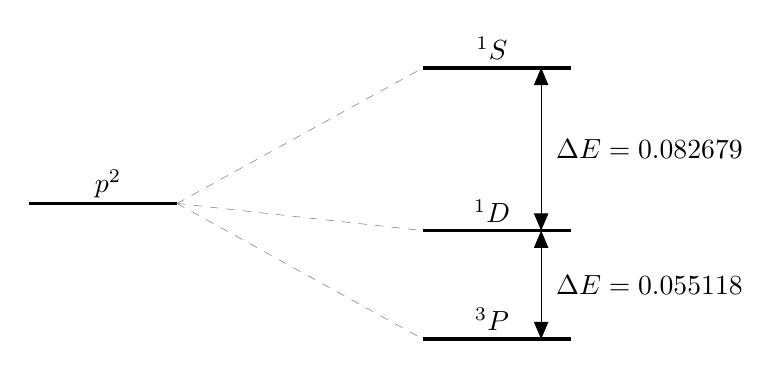
\begin{tikzpicture}[scale=0.125]
  \draw[very thick] (0,13.7797) -- (15,13.7797);
  \draw[very thick] (40,0) -- (55,0);
  \draw[very thick] (40,11.0236) -- (55,11.0236);
  \draw[very thick] (40,27.5594) -- (55,27.5594);
  %
  \node at (8,15.7797) {$p^2$};
  \node at (47,2) {$^3P$};
  \node at (47,13.0236) {$^1D$};
  \node at (47,29.5594) {$^1S$};
  %
  \draw[very thin, gray, dashed] (15,13.7797) -- (40,0);
  \draw[very thin, gray, dashed] (15,13.7797) -- (40,11.0236);
  \draw[very thin, gray, dashed] (15,13.7797) -- (40,27.5594);
  %
  \draw[triangle 45-triangle 45] (52,0) -- (52,11.0236);
  \draw[triangle 45-triangle 45] (52,11.0236) -- (52,27.5594);
  %
  \node at (63,5.5118) {$\Delta E = 0.055118$};
  \node at (63,19.2915) {$\Delta E = 0.082679$};
  \end{tikzpicture}
  \end{center}
  \end{figure}
\end{frame}

\begin{frame}[t]
  \frametitle{JavaScript demonstration}
  \footnotesize
  \centering
  \includegraphics[width=0.8\textwidth]{js2}
  \[\texttt{www.cond-mat.de/sims/multiplet}\]
\end{frame}

\begin{frame}[t]
  \frametitle{Spin-orbit coupling}
  \small
  Our original Hamiltonian
  \[
  H = \sum_{i=1}^N \left[ -\frac{1}{2} \nabla_i^2 - \frac{Z}{r_i} \right] + \sum_{i<j}^N \frac{1}{|\vec{r}_i - \vec{r}_j|}
  \] \pause
  A \emph{magnetic} force?
  \vspace{-1em}
  \begin{center}
  \includegraphics[width=0.4\textwidth]{magnet}
  \end{center}
\end{frame}

\begin{frame}[t]
  \frametitle{Spin-orbit coupling}
  \small
  The Hamiltonian with \emph{spin-orbit} effect
  \[
  H = \sum_{i=1}^N \left[ -\frac{1}{2} \nabla_i^2 - \frac{Z}{r_i} \right] + \sum_{i<j}^N \frac{1}{|\vec{r}_i - \vec{r}_j|} + \underbrace{\sum_{i=1}^N \xi(r_i) \boldsymbol{\ell}_i\cdot\vec{s}_i}_{\emph{\text{Weak}}}
  \]
  where,
  \[ \xi(r) = \frac{1}{2c^2} \frac{1}{r} \frac{dV}{dr} \]
  In atomic units
  \[ c \approx 137.036\ \mathrm{a_0/t_0} \]
\end{frame}

\begin{frame}[t]
  \frametitle{Spin-orbit coupling within multiplet terms}
  \small
  \emph{Clebsch-Grodan} transformation
  \[ \Ket{L,M_L,S,M_S} \rightarrow \Ket{L,S,J,M_J} \]
  Multiplet split
  \[ ^{2S+1}L_J \quad \text{with} \quad J=L+S,L+S-1,\ldots,|L-S| \]
  \[ ^3P \rightarrow {^3P_2},{^3P_1},{^3P_0} \]
  Eigen-energies
  \[\boxed{
  E_\text{SO} = A(nl,LS) \frac{1}{2}[J(J+1)-L(L+1)-S(S+1)]
  }\]
\end{frame}

\begin{frame}[t]
  \frametitle{Spin-orbit coupling within multiplet terms}
  \footnotesize
  Energy splitting
  \vspace{-2em}
  \begin{figure}[h!]
  \begin{center}
  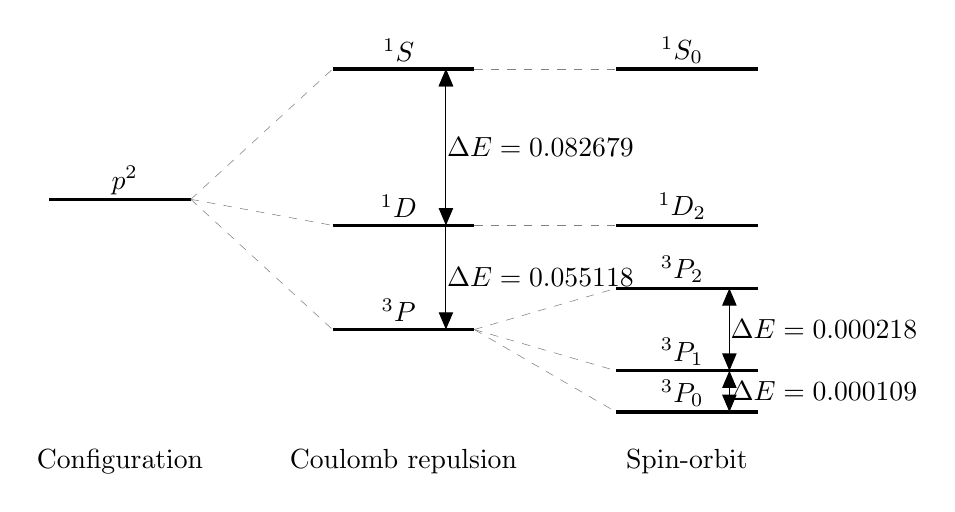
\begin{tikzpicture}[scale=0.12]
  \newcommand{\LA}{0}
  \newcommand{\RA}{15}
  \newcommand{\LB}{30}
  \newcommand{\RB}{45}
  \newcommand{\LC}{60}
  \newcommand{\RC}{75}
  \newcommand{\EA}{13.7797}
  \newcommand{\EBa}{27.5594}
  \newcommand{\EBb}{11.0236}
  \newcommand{\EBc}{0}
  \newcommand{\ECa}{27.5594}
  \newcommand{\ECb}{11.0236}
  \newcommand{\ECc}{ 4.36}
  \newcommand{\ECd}{-4.36}
  \newcommand{\ECe}{-8.72}
  %
  \draw[very thick] (\LA,\EA) -- (\RA,\EA);
  %
  \draw[very thick] (\LB,\EBa) -- (\RB,\EBa);
  \draw[very thick] (\LB,\EBb) -- (\RB,\EBb);
  \draw[very thick] (\LB,\EBc) -- (\RB,\EBc);
  %
  \draw[very thick] (\LC,\ECa) -- (\RC,\ECa);
  \draw[very thick] (\LC,\ECb) -- (\RC,\ECb);
  \draw[very thick] (\LC,\ECc) -- (\RC,\ECc);
  \draw[very thick] (\LC,\ECd) -- (\RC,\ECd);
  \draw[very thick] (\LC,\ECe) -- (\RC,\ECe);
  %
  \node at (\LA+8,\EA+2) {$p^2$};
  \node at (\LB+7,\EBa+2) {$^1S$};
  \node at (\LB+7,\EBb+2) {$^1D$};
  \node at (\LB+7,\EBc+2) {$^3P$};
  \node at (\LC+7,\ECa+2) {$^1S_0$};
  \node at (\LC+7,\ECb+2) {$^1D_2$};
  \node at (\LC+7,\ECc+2) {$^3P_2$};
  \node at (\LC+7,\ECd+2) {$^3P_1$};
  \node at (\LC+7,\ECe+2) {$^3P_0$};
  %
  \draw[very thin, gray, dashed] (\RA,\EA) -- (\LB,\EBa);
  \draw[very thin, gray, dashed] (\RA,\EA) -- (\LB,\EBb);
  \draw[very thin, gray, dashed] (\RA,\EA) -- (\LB,\EBc);
  %
  \draw[very thin, gray, dashed] (\RB,\EBa) -- (\LC,\ECa);
  \draw[very thin, gray, dashed] (\RB,\EBb) -- (\LC,\ECb);
  \draw[very thin, gray, dashed] (\RB,\EBc) -- (\LC,\ECc);
  \draw[very thin, gray, dashed] (\RB,\EBc) -- (\LC,\ECd);
  \draw[very thin, gray, dashed] (\RB,\EBc) -- (\LC,\ECe);
  %
  \draw[triangle 45-triangle 45] (\LB+12,\EBa) -- (\LB+12,\EBb);
  \draw[triangle 45-triangle 45] (\LB+12,\EBa) -- (\LB+12,\EBc);
  \draw[triangle 45-triangle 45] (\LC+12,\ECc) -- (\LC+12,\ECd);
  \draw[triangle 45-triangle 45] (\LC+12,\ECd) -- (\LC+12,\ECe);
  %
  \node at (\RB+7,19.2915) {$\Delta E = 0.082679$};
  \node at (\RB+7,5.5118) {$\Delta E = 0.055118$};
  \node at (\RC+7,0) {$\Delta E = 0.000218$};
  \node at (\RC+7,-6.54) {$\Delta E = 0.000109$};
  %
  \node at (\LA+7.5,-14) {Configuration};
  \node at (\LB+7.5,-14) {Coulomb repulsion};
  \node at (\LC+7.5,-14) {Spin-orbit};
  \end{tikzpicture}
  \end{center}
  \end{figure}
  
  \pause \Put(195,110){\includegraphics[width=0.55\textwidth]{mag}}
\end{frame}

\begin{frame}[t]
  \frametitle{Spin-orbit coupling within entire shell}
  \footnotesize
  \begin{center}
  \vspace{-0.5em}
  \begin{tabular}{|c|c|c|}
  \hline
  $\bullet$ & $\bullet$ & $\phantom{\bullet}$ \\ \hline
  &  &  \\
  \hline
  \end{tabular}
  \begin{tabular}{|c|c|c|}
  \hline
  $\bullet$ & $\phantom{\bullet}$ & $\bullet$ \\ \hline
  &  &  \\
  \hline
  \end{tabular}
  \begin{tabular}{|c|c|c|}
  \hline
  $\bullet$ & $\phantom{\bullet}$ & $\phantom{\bullet}$ \\ \hline
  $\bullet$ &  &  \\
  \hline
  \end{tabular}
  \begin{tabular}{|c|c|c|}
  \hline
  $\bullet$ & $\phantom{\bullet}$ & $\phantom{\bullet}$ \\ \hline
  & $\bullet$ &  \\
  \hline
  \end{tabular}
  \begin{tabular}{|c|c|c|}
  \hline
  $\bullet$ & $\phantom{\bullet}$ & $\phantom{\bullet}$ \\ \hline
  &  & $\bullet$ \\
  \hline
  \end{tabular} \\
  \vspace{0.5em}
  \begin{tabular}{|c|c|c|}
  \hline
  $\phantom{\bullet}$ & $\bullet$ & $\bullet$ \\ \hline
  &  &  \\
  \hline
  \end{tabular}
  \begin{tabular}{|c|c|c|}
  \hline
  $\phantom{\bullet}$ & $\bullet$ & $\phantom{\bullet}$ \\ \hline
  $\bullet$ &  &  \\
  \hline
  \end{tabular}
  \begin{tabular}{|c|c|c|}
  \hline
  $\phantom{\bullet}$ & $\bullet$ & $\phantom{\bullet}$ \\ \hline
  & $\bullet$ &  \\
  \hline
  \end{tabular}
  \begin{tabular}{|c|c|c|}
  \hline
  $\phantom{\bullet}$ & $\bullet$ & $\phantom{\bullet}$ \\ \hline
  &  & $\bullet$ \\
  \hline
  \end{tabular}
  \begin{tabular}{|c|c|c|}
  \hline
  $\phantom{\bullet}$ & $\phantom{\bullet}$ & $\bullet$ \\ \hline
  $\bullet$ &  &  \\
  \hline
  \end{tabular} \\
  \vspace{0.5em}
  \begin{tabular}{|c|c|c|}
  \hline
  $\phantom{\bullet}$ & $\phantom{\bullet}$ & $\bullet$ \\ \hline
  & $\bullet$ &  \\
  \hline
  \end{tabular}
  \begin{tabular}{|c|c|c|}
  \hline
  $\phantom{\bullet}$ & $\phantom{\bullet}$ & $\bullet$ \\ \hline
  &  & $\bullet$ \\
  \hline
  \end{tabular}
  \begin{tabular}{|c|c|c|}
  \hline
  $\phantom{\bullet}$ & $\phantom{\bullet}$ & $\phantom{\bullet}$ \\ \hline
  $\bullet$ & $\bullet$ &  \\
  \hline
  \end{tabular}
  \begin{tabular}{|c|c|c|}
  \hline
  $\phantom{\bullet}$ & $\phantom{\bullet}$ & $\phantom{\bullet}$ \\ \hline
  $\bullet$ &  & $\bullet$ \\
  \hline
  \end{tabular}
  \begin{tabular}{|c|c|c|}
  \hline
  $\phantom{\bullet}$ & $\phantom{\bullet}$ & $\phantom{\bullet}$ \\ \hline
  & $\bullet$ & $\bullet$ \\
  \hline
  \end{tabular}
  \end{center}
  \[ H_\text{SO} = \sum_{i=1}^N \xi(r_i) \boldsymbol{\ell}_i\cdot\vec{s}_i
  \quad \longrightarrow \quad
  H_\text{SO} = \sum_{\alpha,\beta} V_{\alpha\beta} c_\alpha^\dagger c_\beta \]
  
  \[ V_{\alpha\beta} = \Bra{\alpha} \xi(r) \boldsymbol{\ell}\cdot\vec{s} \Ket{\beta} \]
\end{frame}

\begin{frame}[t]
  \frametitle{Spin-orbit coupling within entire shell}
  \footnotesize
  \vspace{-1em}
  \begin{center}
  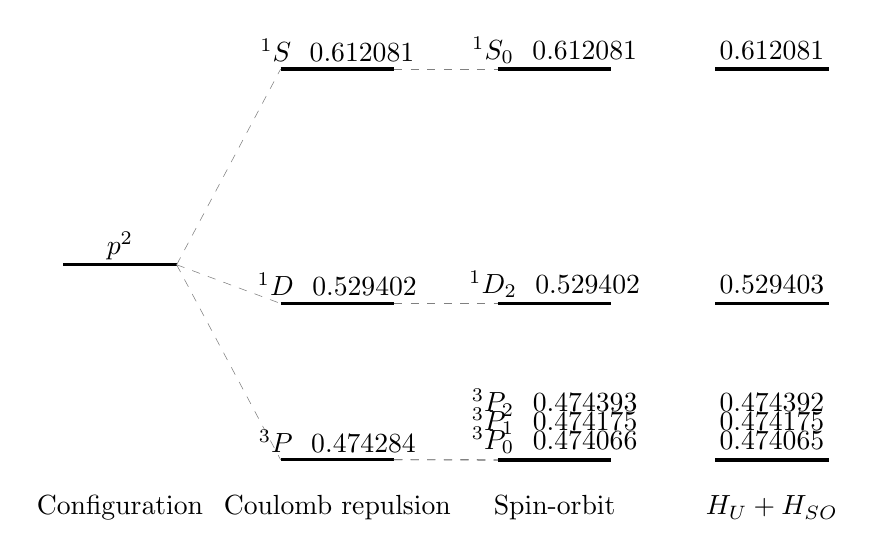
\begin{tikzpicture}[scale=0.12]
  \newcommand{\LA}{0}
  \newcommand{\RA}{12}
  \newcommand{\LB}{23}
  \newcommand{\RB}{35}
  \newcommand{\LC}{46}
  \newcommand{\RC}{58}
  \newcommand{\LD}{69}
  \newcommand{\RD}{81}
  \newcommand{\EA}{13.8016*1.5}
  \newcommand{\EBa}{27.6032*1.5}
  \newcommand{\EBb}{11.0674*1.5}
  \newcommand{\EBc}{0.0438*1.5}
  \newcommand{\ECa}{27.6032*1.5}
  \newcommand{\ECb}{11.0674*1.5}
  \newcommand{\ECc}{0.0656*1.5}
  \newcommand{\ECd}{0.0220*1.5}
  \newcommand{\ECe}{0.0002*1.5}
  \newcommand{\EDa}{27.6032*1.5}
  \newcommand{\EDb}{11.0676*1.5}
  \newcommand{\EDc}{0.0658*1.5}
  \newcommand{\EDd}{0.0220*1.5}
  \newcommand{\EDe}{0.0000*1.5}
  %
  \draw[very thick] (\LA,\EA) -- (\RA,\EA);
  %
  \draw[very thick] (\LB,\EBa) -- (\RB,\EBa);
  \draw[very thick] (\LB,\EBb) -- (\RB,\EBb);
  \draw[very thick] (\LB,\EBc) -- (\RB,\EBc);
  %
  \draw[very thick] (\LC,\ECa) -- (\RC,\ECa);
  \draw[very thick] (\LC,\ECb) -- (\RC,\ECb);
  \draw[very thick] (\LC,\ECc) -- (\RC,\ECc);
  \draw[very thick] (\LC,\ECd) -- (\RC,\ECd);
  \draw[very thick] (\LC,\ECe) -- (\RC,\ECe);
  %
  \draw[very thick] (\LD,\EDa) -- (\RD,\EDa);
  \draw[very thick] (\LD,\EDb) -- (\RD,\EDb);
  \draw[very thick] (\LD,\EDc) -- (\RD,\EDc);
  \draw[very thick] (\LD,\EDd) -- (\RD,\EDd);
  \draw[very thick] (\LD,\EDe) -- (\RD,\EDe);
  %
  \draw[very thin, gray, dashed] (\RA,\EA) -- (\LB,\EBa);
  \draw[very thin, gray, dashed] (\RA,\EA) -- (\LB,\EBb);
  \draw[very thin, gray, dashed] (\RA,\EA) -- (\LB,\EBc);
  %
  \draw[very thin, gray, dashed] (\RB,\EBa) -- (\LC,\ECa);
  \draw[very thin, gray, dashed] (\RB,\EBb) -- (\LC,\ECb);
  \draw[very thin, gray, dashed] (\RB,\EBc) -- (\LC,\ECc);
  \draw[very thin, gray, dashed] (\RB,\EBc) -- (\LC,\ECd);
  \draw[very thin, gray, dashed] (\RB,\EBc) -- (\LC,\ECe);
  %
  \node at (\LA+6,\EA+2) {$p^2$};
  \node at (\LB+6,\EBa+2) {$^1S\ $ 0.612081};
  \node at (\LB+6,\EBb+2) {$^1D\ $ 0.529402};
  \node at (\LB+6,\EBc+2) {$^3P\ $ 0.474284};
  \node at (\LC+6,\ECa+2) {$^1S_0\ $ 0.612081};
  \node at (\LC+6,\ECb+2) {$^1D_2\ $ 0.529402};
  \node at (\LC+6,\ECc+6) {$^3P_2\ $ 0.474393};
  \node at (\LC+6,\ECc+4) {$^3P_1\ $ 0.474175};
  \node at (\LC+6,\ECc+2) {$^3P_0\ $ 0.474066};
  \node at (\LD+6,\EDa+2) {0.612081};
  \node at (\LD+6,\EDb+2) {0.529403};
  \node at (\LD+6,\EDc+6) {0.474392};
  \node at (\LD+6,\EDc+4) {0.474175};
  \node at (\LD+6,\EDc+2) {0.474065};
  %
  \node at (\LA+6,-5) {Configuration};
  \node at (\LB+6,-5) {Coulomb repulsion};
  \node at (\LC+6,-5) {Spin-orbit};
  \node at (\LD+6,-5) {$H_U+H_\text{SO}$};
  \end{tikzpicture}
  \end{center}
  
  \Put(23,320){$\emph{\Huge \boxed{\text{C}}}$}
\end{frame}

\begin{frame}[t]
  \frametitle{Spin-orbit coupling within entire shell}
  \footnotesize
  \vspace{-0.8em}
  \begin{center}
  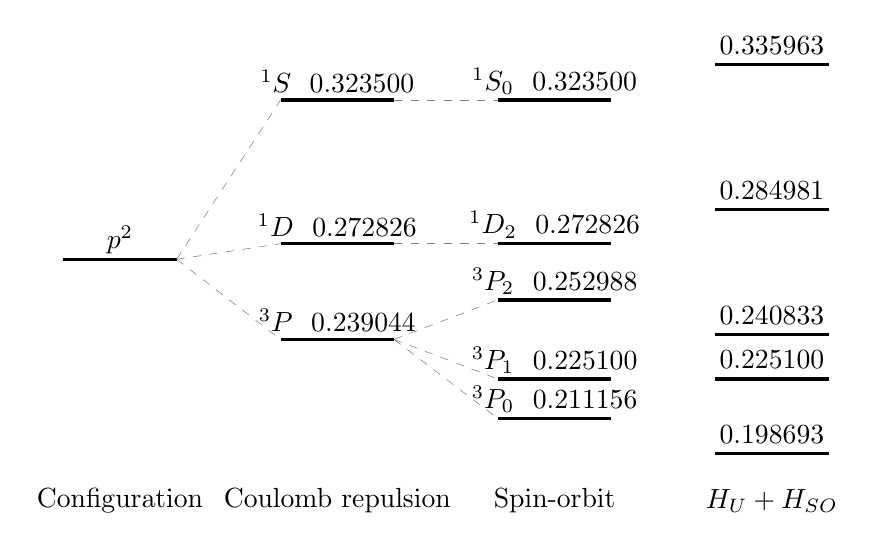
\begin{tikzpicture}[scale=0.12]
  \newcommand{\LA}{0}
  \newcommand{\RA}{12}
  \newcommand{\LB}{23}
  \newcommand{\RB}{35}
  \newcommand{\LC}{46}
  \newcommand{\RC}{58}
  \newcommand{\LD}{69}
  \newcommand{\RD}{81}
  \newcommand{\EA}{13.7270*1.5}
  \newcommand{\EBa}{24.9614*1.5}
  \newcommand{\EBb}{14.8266*1.5}
  \newcommand{\EBc}{ 8.0702*1.5}
  \newcommand{\ECa}{24.9614*1.5}
  \newcommand{\ECb}{14.8266*1.5}
  \newcommand{\ECc}{10.8590*1.5}
  \newcommand{\ECd}{ 5.2814*1.5}
  \newcommand{\ECe}{ 2.4926*1.5}
  \newcommand{\EDa}{27.4540*1.5}
  \newcommand{\EDb}{17.2576*1.5}
  \newcommand{\EDc}{ 8.4280*1.5}
  \newcommand{\EDd}{ 5.2814*1.5}
  \newcommand{\EDe}{ 0.0000*1.5}
  %
  \draw[very thick] (\LA,\EA) -- (\RA,\EA);
  %
  \draw[very thick] (\LB,\EBa) -- (\RB,\EBa);
  \draw[very thick] (\LB,\EBb) -- (\RB,\EBb);
  \draw[very thick] (\LB,\EBc) -- (\RB,\EBc);
  %
  \draw[very thick] (\LC,\ECa) -- (\RC,\ECa);
  \draw[very thick] (\LC,\ECb) -- (\RC,\ECb);
  \draw[very thick] (\LC,\ECc) -- (\RC,\ECc);
  \draw[very thick] (\LC,\ECd) -- (\RC,\ECd);
  \draw[very thick] (\LC,\ECe) -- (\RC,\ECe);
  %
  \draw[very thick] (\LD,\EDa) -- (\RD,\EDa);
  \draw[very thick] (\LD,\EDb) -- (\RD,\EDb);
  \draw[very thick] (\LD,\EDc) -- (\RD,\EDc);
  \draw[very thick] (\LD,\EDd) -- (\RD,\EDd);
  \draw[very thick] (\LD,\EDe) -- (\RD,\EDe);
  %
  \draw[very thin, gray, dashed] (\RA,\EA) -- (\LB,\EBa);
  \draw[very thin, gray, dashed] (\RA,\EA) -- (\LB,\EBb);
  \draw[very thin, gray, dashed] (\RA,\EA) -- (\LB,\EBc);
  %
  \draw[very thin, gray, dashed] (\RB,\EBa) -- (\LC,\ECa);
  \draw[very thin, gray, dashed] (\RB,\EBb) -- (\LC,\ECb);
  \draw[very thin, gray, dashed] (\RB,\EBc) -- (\LC,\ECc);
  \draw[very thin, gray, dashed] (\RB,\EBc) -- (\LC,\ECd);
  \draw[very thin, gray, dashed] (\RB,\EBc) -- (\LC,\ECe);
  %
  \node at (\LA+6,\EA+2) {$p^2$};
  \node at (\LB+6,\EBa+2) {$^1S\ $ 0.323500};
  \node at (\LB+6,\EBb+2) {$^1D\ $ 0.272826};
  \node at (\LB+6,\EBc+2) {$^3P\ $ 0.239044};
  \node at (\LC+6,\ECa+2) {$^1S_0\ $ 0.323500};
  \node at (\LC+6,\ECb+2) {$^1D_2\ $ 0.272826};
  \node at (\LC+6,\ECc+2) {$^3P_2\ $ 0.252988};
  \node at (\LC+6,\ECd+2) {$^3P_1\ $ 0.225100};
  \node at (\LC+6,\ECe+2) {$^3P_0\ $ 0.211156};
  \node at (\LD+6,\EDa+2) {0.335963};
  \node at (\LD+6,\EDb+2) {0.284981};
  \node at (\LD+6,\EDc+2) {0.240833};
  \node at (\LD+6,\EDd+2) {0.225100};
  \node at (\LD+6,\EDe+2) {0.198693};
  %
  \node at (\LA+6,-5) {Configuration};
  \node at (\LB+6,-5) {Coulomb repulsion};
  \node at (\LC+6,-5) {Spin-orbit};
  \node at (\LD+6,-5) {$H_U+H_\text{SO}$};
  \end{tikzpicture}
  \end{center}
  
  \Put(17,320){$\emph{\Huge \boxed{\text{Pb}}}$}
\end{frame}
\begin{frame}[t]
  \frametitle{Conclusion}
  \small
  \begin{enumerate}
    \item We implemented Numerov's method with logarithmic grid to solve
    the \emph{one-electron} problem and obtained very accurate solutions.
    \item We solved the many-electron problem using \emph{self-consistent field} approximation.
    \item Based on SCF calculation, we constructed atomic \emph{multiplet states},
    which are the many-electron eigen-states in atoms.
    \item Finally we introduced the \emph{spin-orbit coupling}, where we see the
    spectral lines further split into finer structures.
  \end{enumerate}
\end{frame}

\begin{frame}[t]
  \begin{center}
    \Huge \emph{Thank You!}
  \end{center}
    Special thanks to: \newline
  \begin{itemize}
    \item {Prof.\ Dr.\ Erik Koch}
    \item {Dr.\ Hermann Ulm}
    \item {German Research School for Simulation Sciences}
    \item {Forschungszentrum J\"{u}lich GmbH}
  \end{itemize}
\end{frame}
\begin{frame}[t]
  \vspace{5em}
  \begin{center}
    \Huge \emph{Backup Materials}
  \end{center}
\end{frame}

\begin{frame}[t]
  \frametitle{Numerov's method}
  \footnotesize
  Finite difference
  \[\frac{d^2\tilde{u}}{dx^2} = \frac{\tilde{u}_{i+1} - 2\tilde{u}_i + \tilde{u}_{i-1}}{\Delta x^2} + \mathcal{O}(\Delta x^2)\]
  \emph{Numerov's method}
  \[\frac{d^2\tilde{u}}{dx^2} = \frac{\tilde{u}_{i+1} - 2\tilde{u}_i + \tilde{u}_{i-1}}{\Delta x^2} - \frac{1}{12}\frac{\tilde{u}_{i+1}^{''} - 2\tilde{u}_i^{''} + \tilde{u}_{i-1}^{''}}{\Delta x^2}\Delta x^2 + \mathcal{O}(\Delta x^4)\]
  Use the original ODE
  \[\tilde{u}_i^{''} = -2 k_i^2 \tilde{u_i}
  \quad \text{and} \quad k_i^2 \equiv r_i^2 E - r_i^2 V(r_i) - \frac{1}{2} \Big(l+\frac{1}{2}\Big)^2\]
  3-point \alert{recursion}!
  \[\tilde{u}_{i\pm1} = \frac{(2-\frac{5\Delta x^2}{3}k_i^2)\tilde{u}_i - (1+\frac{\Delta x^2}{6}k_{i\mp1}^2)\tilde{u}_{i\mp1}}{1+\frac{\Delta x^2}{6}k_{i\pm1}^2}\]
\end{frame}

\begin{frame}[t]
  \frametitle{Slater-Condon parameters}
  \footnotesize
  \vspace{-2em}
  \[
  R^{(k)}(n_1l_1,n_2l_2,n_3l_3,n_4l_4) =
  \int_0^\infty dr_1 \int_0^\infty dr_2\, \conj{u_{n_1l_1}}(r_1) \conj{u_{n_2l_2}}(r_2)
  \frac{r_<^k}{r_>^{k+1}} u_{n_3l_3}(r_2) u_{n_4l_4}(r_1)
  \]
  If $r_1 \le r_2$,
  \[
    \begin{array}{c c}
    r_<=r_1, & r_>=r_2
    \end{array}
  \]
  If $r_1 > r_2$,
  \[
    \begin{array}{c c}
    r_<=r_2, & r_>=r_1
    \end{array}
  \]
  $R^{(k)}(n_1l_1,n_2l_2,n_3l_3,n_4l_4) = $
  \[
  \begin{aligned}
  & \int_0^\infty dr_1
  \conj{u_{n_1l_1}}(r_1)u_{n_4l_4}(r_1)
  \left[ \frac{1}{r_1^{k+1}} \int_0^{r_1} dr_2\, r_2^k \conj{u_{n_2l_2}}(r_2)u_{n_3l_3}(r_2) \right. \\
  & \qquad\qquad\qquad\qquad\qquad\quad
  \left. + r_1^k \int_{r_1}^\infty dr_2\, \frac{1}{r_2^{k+1}} \conj{u_{n_2l_2}}(r_2)u_{n_3l_3}(r_2) \right]
  \end{aligned}
  \]
\end{frame}

\begin{frame}[t]
  \frametitle{Gaunt coefficients}
  \footnotesize
  $A^{(k)}(l_1m_1,l_2m_2,l_3m_3,l_4m_4) =$
  \begin{align*}
  \sum_{\mu=-k}^k
  & \int_0^{2\pi}d\phi_1 \int_0^{\pi}d\theta_1\,\sin{\theta_1}\,
    \conj{Y_{l_1m_1}}(\theta_1,\phi_1) \conj{Y_{k\mu}}(\theta_1,\phi_1) Y_{l_4m_4}(\theta_1,\phi_1) \nonumber \\
  & \int_0^{2\pi}d\phi_2 \int_0^{\pi}d\theta_2\,\sin{\theta_2}\,
    \conj{Y_{l_2m_2}}(\theta_2,\phi_2) Y_{k\mu}(\theta_2,\phi_2) Y_{l_3m_3}(\theta_2,\phi_2)
  \end{align*}
  
  \vspace{1em}
  \emph{Gaunt coefficients}
  \[g_{m_1m_2}^{(k)} = \Bra{l_1m_1} k\mu \Ket{l_2m_2}\]
\end{frame}

\begin{frame}[t]
  \frametitle{Gaunt coefficients}
  \scriptsize
  \emph{Recursion} relation
  
  \vspace{1em}
  $\Bra{l_1m_1} k\mu \Ket{l_2m_2} = $
  \vspace{-0.5em}
  \[ a \Bra{l_1+1,m_1} k-1,\mu \Ket{l_2m_2}
  + b \Bra{l_1-1,m_1} k-1,\mu \Ket{l_2m_2}
  + c \Bra{l_1m_1} k-2,\mu \Ket{l_2m_2}
  \]
  \vspace{-2em}
  \begin{align*}
  a & = \sqrt{\frac{(2k+1)(2k-1)(l_1+m_1+1)(l_1-m_1+1)}{(k+\mu)(k-\mu)(2l_1+3)(2l_1+1)}} \\
  b & = \sqrt{\frac{(2k+1)(2k-1)(l_1+m_1)(l_1-m_1)}{(k+\mu)(k-\mu)(2l_1+1)(2l_1-1)}} \\
  c & = -\sqrt{\frac{(2k+1)(k+\mu-1)(k-\mu-1)}{(k+\mu)(k-\mu)(2k-3)}}
  \end{align*}
  \emph{Base} case
  \[\Bra{l_1m_1} 00 \Ket{l_2m_2} = \frac{1}{\sqrt{4\pi}} \delta_{l_1l_2} \delta_{m_1m_2}\]
\end{frame}

\begin{frame}[t]
  \frametitle{Ladder operator techniques}
  \scriptsize
  \emph{Ladder operators}
  \[ L_\pm \Ket{lm} = \alpha_{lm}^\pm \Ket{l,m\pm1} \]
  
  \vspace{-2.5em}
  \begin{align*}
  \alpha_{lm}^+ & = \sqrt{(l+m+1)(l-m)} \\
  \alpha_{lm}^- & = \sqrt{(l+m)(l-m+1)}
  \end{align*}
  Express \emph{eigen-vectors} in terms of our 15 \emph{basis vectors}
  \begin{align*}
  L_-
  \begin{array}{|c|c|c|}
  \hline
  \bullet & \phantom{\bullet} & \phantom{\bullet} \\ \hline
  \bullet &  &  \\
  \hline
  \end{array} & =
  \sqrt{(1+1)(1-1+1)}
  \begin{array}{|c|c|c|}
  \hline
  \phantom{\bullet} & \bullet & \phantom{\bullet} \\ \hline
  \bullet &  &  \\
  \hline
  \end{array} +
  \sqrt{(1+1)(1-1+1)}
  \begin{array}{|c|c|c|}
  \hline
  \bullet & \phantom{\bullet} & \phantom{\bullet} \\ \hline
  & \bullet &  \\
  \hline
  \end{array} \nonumber \\
  L_-\Ket{2,2,0,0} & = \qquad \qquad \qquad \qquad
  \sqrt{2}\:
  \begin{array}{|c|c|c|}
  \hline
  \phantom{\bullet} & \bullet & \phantom{\bullet} \\ \hline
  \bullet &  &  \\
  \hline
  \end{array} + \qquad \qquad \qquad \qquad
  \sqrt{2}\:
  \begin{array}{|c|c|c|}
  \hline
  \bullet & \phantom{\bullet} & \phantom{\bullet} \\ \hline
  & \bullet &  \\
  \hline
  \end{array} \nonumber \\
  \Ket{2,1,0,0} & = \qquad \qquad \qquad \qquad
  \frac{1}{\sqrt{2}}
  \begin{array}{|c|c|c|}
  \hline
  \phantom{\bullet} & \bullet & \phantom{\bullet} \\ \hline
  \bullet &  &  \\
  \hline
  \end{array} + \qquad \qquad \qquad \qquad
  \frac{1}{\sqrt{2}}
  \begin{array}{|c|c|c|}
  \hline
  \bullet & \phantom{\bullet} & \phantom{\bullet} \\ \hline
  & \bullet &  \\
  \hline
  \end{array} \\
  \Ket{2,1,0,0} & = \qquad \qquad \qquad \qquad
  \frac{1}{\sqrt{2}} \ \ \ c_{1\downarrow}^\dagger c_{0\uparrow}^\dagger \Ket{0} \ \
  + \qquad \qquad \qquad \qquad
  \frac{1}{\sqrt{2}} \ \ \ c_{0\downarrow}^\dagger c_{1\uparrow}^\dagger \Ket{0}
  \end{align*}
\end{frame}



\end{document}
